\documentclass[12pt]{article}
\usepackage[utf8]{inputenc}
\usepackage[brazilian]{babel}
\usepackage{enumitem}
\usepackage{graphicx}

\graphicspath{{fig/}}

\author{Gabriel de Paula e Lima  587710\\
        Giovana Vieira de Morais  587591}
\title{Relatório Projeto 3}
\begin{document}

\maketitle
\newpage

\section*{A atividade}

\begin{itemize}
    \item{Compilar o módulo fornecido como exemplo}
    \item{Modificar o módulo fornecido para exibir, no lugar da frase fixa,
    o PID do processo lendo o arquivo e o PID do seu processo pai}
    \item{Dar ao interpretador de comando executando o processo de leitura
        permissões de root}
\end{itemize}

\subsection*{Exibir o PID do processo lendo o arquivo (\texttt{cat}) e do
processo pai(\texttt{bash})}
    Para essa função, foi necessário usar a task\_struct, que é uma struct que
    descreve informações de processos ou tarefas do sistema, guardando
    informações importantes como PID, nome do processo atual, credenciais do
    grupo e do processo e processo pai.

    Após a declaração de um ponteiro para a estrutura, só foi necessário
    imprimir o nome (\texttt{task->comm}) e o pid (\texttt{task->pid}) do
    processo atual. Para imprimir as informações do processo pai:
    \texttt{task->parent->comm} e \texttt{task->parent->pid}.
\subsection*{Dar ao processo pai permissões de root}
    Assim como mencionado acima, a \texttt{task\_struct} contém em suas
    informações as credenciais do usuário e do grupo. As credenciais
    especificadamente ficam definidas dentro da estrutura de dados \texttt{cred}.
    Para darmos permissão de root ao processo pai,nesse caso o (\texttt{bash}),
    precisamos alterar o \texttt{euid} a qual é a variavel definidora do
    tipo de permissão do processo. Porém não podemos alterá-la diretamente,
    então necessitamos criar uma \texttt{struct} cred, a qual nos permitirá
    alterar as credenciais do processo. Então usamos a função \texttt{get\_cred},
    função esta que retornará ao cred do processo um ponteiro editável
    por meio da struct criada por nós, aí alteramos esse ponteiro editável
    para o valor 0 que é o valor de permissão root e então usamos \texttt{put\_cred},
    o qual sacramenta a edição e subsequente mudança de permissão do processo para acesso root.
\subsection*{Dificuldades encontradas}
    Inicialmente tivemos dificuldade em entender o que nos era pedido
    para realizar, tais dúvidas foram sanadas por meio de
    questionamentos ao professor e leitura de manuais sobre as estruturas
    a serem alteradas para realizar o trabalho. Posteriomente tivemos dificuldade
    em definir se o \texttt{euid} ou o \texttt{uid} deveriam ser alterados
    a fim de dar permissão de root ao usuário, chegando a conclusão por meio
    de pesquisas de que o \texttt{euid} deveria ser alterado. Pois ele diz respeito
    as permissões do processo em si enquanto o \texttt{uid} diz respeito as
    permissões do usuário. Incluisve a primeira versão foi feita alterando o
    \texttt{uid} como mostra a imagem abaixo.
    \newline

    \begin{figure}[h]
      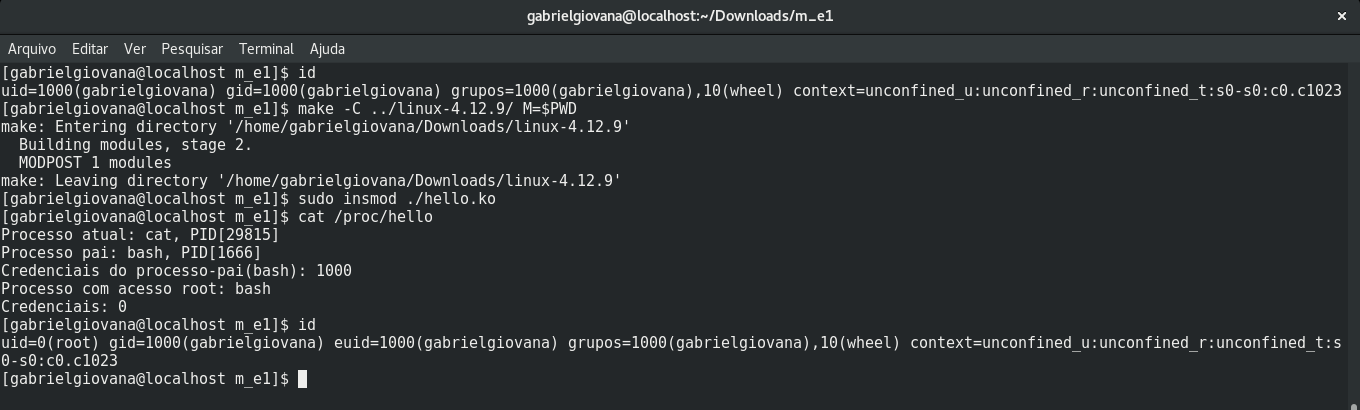
\includegraphics[width=\textwidth]{print}
      \centering
    \end{figure}

\end{document}
